% LeWAM short deck: WAM related-work landscape + LeWAM novelty/goal.
% Anonymous. Cite-keys verbatim from proposal/lewam_refs.bib.
% Compile: pdflatex lewam_short.tex  (twice).
\documentclass[aspectratio=169,10pt]{beamer}
\usetheme{default}
\usecolortheme{seahorse}
\setbeamertemplate{navigation symbols}{}
\setbeamertemplate{footline}[frame number]
\setbeamertemplate{itemize items}[circle]
\usepackage{amsmath}
\usepackage{booktabs}
\usepackage{tikz}
\usetikzlibrary{positioning,arrows.meta,backgrounds,fit,shapes.geometric}

% --- palette ---
\definecolor{video}{RGB}{198,120,40}
\definecolor{latent}{RGB}{40,110,160}
\definecolor{ours}{RGB}{170,30,60}
\definecolor{sidegray}{RGB}{120,120,120}
\definecolor{panel}{RGB}{245,245,248}

% --- reusable node styles for the landscape map ---
\tikzset{
  method/.style={font=\scriptsize, inner sep=2pt, align=center},
  vidnode/.style={method, text=video},
  latnode/.style={method, text=latent},
  ournode/.style={method, text=ours, font=\scriptsize\bfseries},
  sidenode/.style={method, text=sidegray, font=\tiny},
  axislab/.style={font=\footnotesize\bfseries},
  endlab/.style={font=\scriptsize\itshape, text=black!70},
}

\title[LeWAM]{LeWAM: A Simple, Fast, Scalable World--Action Model}
\subtitle{Related work + our goal}
\date{}
\author{}
\institute{}

\begin{document}

\frame[plain]{\titlepage}

% =====================================================================
% SLIDE 1 -- WAM related-work landscape (FIGURE-DENSE)
% =====================================================================
\begin{frame}{The world--action model (WAM) landscape}
\vspace{-2mm}
\begin{center}
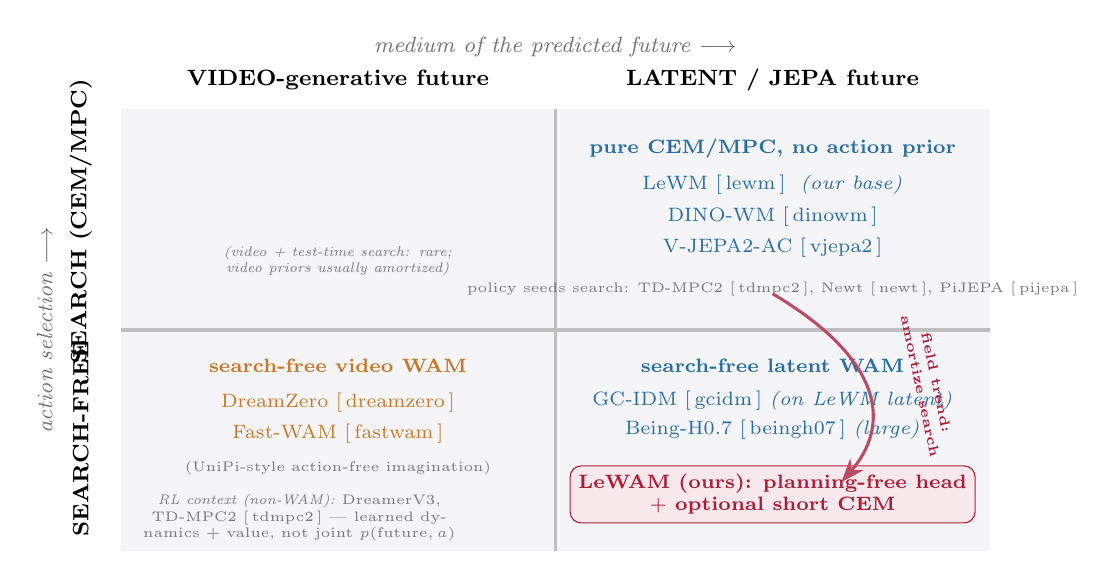
\begin{tikzpicture}[scale=0.92]
  % --- quadrant frame ---
  \def\xmin{0} \def\xmax{12} \def\ymin{0} \def\ymax{6.1}
  \begin{scope}[on background layer]
    \fill[panel] (\xmin,\ymin) rectangle (\xmax,\ymax);
  \end{scope}
  % quadrant divider lines
  \draw[black!25, very thick] (6,\ymin) -- (6,\ymax);
  \draw[black!25, very thick] (\xmin,3.05) -- (\xmax,3.05);

  % --- axes labels ---
  % x-axis: medium of the future
  \node[axislab] at (3, \ymax+0.40) {VIDEO-generative future};
  \node[axislab] at (9, \ymax+0.40) {LATENT / JEPA future};
  \node[font=\footnotesize\itshape, text=black!55] at (6, \ymax+0.86) {medium of the predicted future $\longrightarrow$};
  % y-axis: action selection
  \node[axislab, rotate=90] at (\xmin-0.55, 4.55) {SEARCH (CEM/MPC)};
  \node[axislab, rotate=90] at (\xmin-0.55, 1.55) {SEARCH-FREE};
  \node[font=\footnotesize\itshape, text=black!55, rotate=90] at (\xmin-1.05, 3.05)
       {action selection $\longrightarrow$};

  % ===== TOP-LEFT: video + search (sparse; mostly empty) =====
  \node[sidenode, text width=4.6cm] at (3, 4.0)
    {\textit{(video + test-time search: rare; video priors usually amortized)}};

  % ===== TOP-RIGHT: latent + search -- the classic latent planners =====
  \node[latnode] at (9, 5.55) {\textbf{pure CEM/MPC, no action prior}};
  \node[latnode] at (9, 5.05) {LeWM~[\,lewm\,]~~\textit{(our base)}};
  \node[latnode] at (9, 4.62) {DINO-WM~[\,dinowm\,]};
  \node[latnode] at (9, 4.19) {V-JEPA2-AC~[\,vjepa2\,]};
  \node[latnode, text=sidegray] at (9, 3.62)
    {\tiny policy seeds search: TD-MPC2~[\,tdmpc2\,], Newt~[\,newt\,], PiJEPA~[\,pijepa\,]};

  % ===== BOTTOM-LEFT: video + search-free =====
  \node[vidnode] at (3, 2.55) {\textbf{search-free video WAM}};
  \node[vidnode] at (3, 2.05) {DreamZero~[\,dreamzero\,]};
  \node[vidnode] at (3, 1.62) {Fast-WAM~[\,fastwam\,]};
  \node[vidnode, text=sidegray] at (3, 1.15) {\tiny (UniPi-style action-free imagination)};

  % ===== BOTTOM-RIGHT: latent + search-free =====
  \node[latnode] at (9, 2.55) {\textbf{search-free latent WAM}};
  \node[latnode] at (9, 2.08) {GC-IDM~[\,gcidm\,]~\textit{(on LeWM latent)}};
  \node[latnode] at (9, 1.68) {Being-H0.7~[\,beingh07\,]~\textit{(large)}};

  % ===== OURS: latent, search-free + optional short search (straddle) =====
  \node[ournode, fill=ours!10, draw=ours, rounded corners, inner sep=3pt] (lewam) at (9, 0.78)
    {LeWAM~(ours): planning-free head\\$+$ optional short CEM};

  % --- TREND arrow: field converging toward search-free / amortized ---
  \draw[-{Stealth[length=3mm]}, ours!80, line width=1.1pt]
    (9, 3.55) .. controls (10.6,2.6) and (10.6,1.7) .. (9.95,0.95);
  \node[font=\tiny\bfseries, text=ours, align=center, rotate=-78] at (11.15,2.3)
    {field trend:\\amortize search};

  % --- side note: non-JEPA RL context ---
  \node[sidenode, text width=4.2cm, anchor=south west] at (\xmin+0.1, \ymin+0.05)
    {\textit{RL context (non-WAM):} DreamerV3, TD-MPC2~[\,tdmpc2\,] --- learned dynamics + value, not joint $p(\text{future},a)$};
\end{tikzpicture}
\end{center}
\vspace{-1mm}
{\scriptsize\textbf{Map.} A WAM jointly models $p(\text{future},\,a)$. Axes: future medium (video$\leftrightarrow$latent) $\times$ action selection (test-time search$\leftrightarrow$amortized one forward pass). The field is converging toward \textbf{search-free}. LeWAM is a \textbf{latent} WAM built on LeWM, planning-free by default with optional short search.}
\end{frame}

% =====================================================================
% RELATED WORK (DETAIL) -- one slide per category
% =====================================================================

% --- RW-1: video-generative WAMs ---
\begin{frame}{Related work I --- video-generative WAMs}
\footnotesize
The future is a \textbf{video}: a generative model predicts pixels, actions come from the imagined rollout.
\vspace{4pt}

\begin{itemize}\setlength\itemsep{4pt}
  \item \textbf{DreamZero}~[\,dreamzero\,] --- video diffusion world model $+$ inverse-dynamics action read-out; search-free at test time.
  \item \textbf{Being-H0.7}~[\,beingh07\,] --- large-scale latent/video world-action model trained from egocentric video.
  \item \textbf{UniPi}~[\,unipi\,] --- text-conditioned video generation as a universal policy; inverse dynamics maps frames to actions.
\end{itemize}

\vspace{6pt}
{\color{video}\textbf{Strength.}} Search-free action read-out; scales with web-scale video and pretrained generators.

\vspace{3pt}
{\color{black!75}\textbf{Cost.}} Heavy generative rollouts (full-frame diffusion per step); large data and compute budgets; pixel prediction spends capacity on visual detail irrelevant to control.
\end{frame}

% --- RW-2: latent WAMs with search ---
\begin{frame}{Related work II --- latent WAMs with test-time search}
\footnotesize
The future is a \textbf{latent}: a JEPA-style predictor rolls forward in embedding space; actions are chosen by planning (CEM/MPC) over that predictor.
\vspace{4pt}

\begin{itemize}\setlength\itemsep{4pt}
  \item \textbf{LeWM}~[\,lewm\,] \emph{(our base)} --- stable end-to-end JEPA world model from pixels; learnable encoder, action-conditioned latent predictor.
  \item \textbf{DINO-WM}~[\,dinowm\,] --- world model on frozen DINO features; zero-shot planning by latent rollout.
  \item \textbf{V-JEPA2-AC}~[\,vjepa2\,] --- action-conditioned video JEPA; latent prediction for planning.
\end{itemize}

\vspace{6pt}
{\color{latent}\textbf{Strength.}} Light latent prediction (no pixel decode); strong goal-reaching by optimizing actions against the predictor.

\vspace{3pt}
{\color{black!75}\textbf{Gap.}} \textbf{No learned action prior.} Every step re-samples actions \emph{blind} (CEM population $\times$ horizon $\times$ iterations), paying the full search cost at deployment.
\end{frame}

% --- RW-3: search-free / amortized policies ---
\begin{frame}{Related work III --- search-free / amortized policies}
\footnotesize
Amortize the planner into a network: one forward pass replaces test-time search.
\vspace{4pt}

\begin{itemize}\setlength\itemsep{4pt}
  \item \textbf{GC-IDM}~[\,gcidm\,] --- goal-conditioned inverse dynamics on the LeWM latent; $\sim$100--130$\times$ cheaper than CEM. \emph{Markovian: single-frame $(z_t, z_g, h)$.}
  \item \textbf{Fast-WAM}~[\,fastwam\,] --- argues a world-action model needs \emph{no} test-time future imagination.
  \item Diffusion-policy context --- \textbf{Diffuser}~[\,diffuser\,], \textbf{Decision-Diffuser}~[\,decisiondiffuser\,], \textbf{BESO}~[\,beso\,]: generative trajectory/action heads, no latent-WM rollout.
\end{itemize}

\vspace{6pt}
{\color{latent}\textbf{Strength.}} One forward pass per action; deployment-cheap.

\vspace{3pt}
{\color{black!75}\textbf{Note.}} GC-IDM conditions on a \emph{single} frame (Markovian); diffusion heads add $K$ denoising steps and do not reuse a world-model predictor.
\end{frame}

% =====================================================================
% DIFFERENCE -- previous work vs LeWAM (the explicit contrast)
% =====================================================================
\begin{frame}{Previous work vs LeWAM}
\scriptsize
\setlength{\tabcolsep}{4pt}\renewcommand{\arraystretch}{1.25}
\begin{tabular}{@{}p{3.0cm} p{5.2cm} p{4.6cm}@{}}
\toprule
\textbf{Prior family} & \textbf{What they do / limit} & \textbf{What LeWAM does differently} \\
\midrule
Pure-CEM latent WMs\newline LeWM~[\,lewm\,], DINO-WM~[\,dinowm\,], V-JEPA2-AC~[\,vjepa2\,] &
Search \emph{blind} at every step; no learned action prior. &
Adds a planning-free action head $\Rightarrow$ \textbf{$\sim$1104$\times$ fewer FLOPs/action} (measured); keep search only where it helps. \\
\addlinespace
Amortized GC-IDM\newline GC-IDM~[\,gcidm\,] &
One forward pass, but \emph{Markovian} (single frame); one control mode. &
\textbf{History-conditioned} head; \textbf{one model unifies three settings} (planning / goal-conditioned / BC). \\
\addlinespace
Video-generative WAMs\newline DreamZero~[\,dreamzero\,], Being-H0.7~[\,beingh07\,] &
Heavy generative rollouts; large data/compute. &
\textbf{Light vit-tiny latent}; no pixel decode, no generative rollout. \\
\bottomrule
\end{tabular}

\vspace{5pt}
\hrule height 0.4pt
\vspace{4pt}
{\footnotesize\textbf{Honest positioning.} LeWAM's contribution is the \textbf{efficiency Pareto}, the \textbf{multi-setting per-family analysis}, and being built on LeWM~[\,lewm\,] --- \emph{not} a state-of-the-art success rate.}
\end{frame}

% =====================================================================
% SLIDE 2 -- LeWAM novelty + schematic
% =====================================================================
\begin{frame}{LeWAM = LeWM latent $+$ a planning-free action head}
\begin{columns}[T]
\begin{column}{0.49\textwidth}
\footnotesize
\textbf{One trained model, three control settings.}
\begin{itemize}\setlength\itemsep{3pt}
  \item \textbf{Base:} LeWM~[\,lewm\,] --- stable end-to-end JEPA world model from pixels (learnable encoder, action-conditioned predictor).
  \item \textbf{Ours:} a history/goal/horizon-conditioned \textbf{action head} trained jointly on the same latent.
  \item Decodes into 3 settings without retraining: \emph{planning} (predictor $+$ CEM), \emph{goal-conditioned policy}, \emph{behavior cloning}.
\end{itemize}
\vspace{2pt}
\textbf{What is ours} (honest scope): the action head, the efficiency result, and the per-setting analysis. The base WM is LeWM. No SOTA success-rate claim.
\end{column}

\begin{column}{0.51\textwidth}
\centering
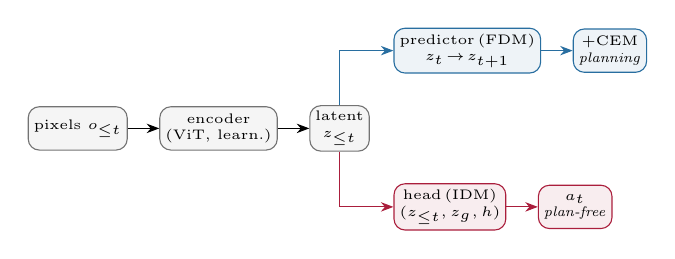
\begin{tikzpicture}[font=\tiny, node distance=3mm and 4mm,
   box/.style={draw, rounded corners, align=center, inner sep=2pt, minimum height=5.5mm},
   fdm/.style={box, draw=latent, fill=latent!8},
   idm/.style={box, draw=ours, fill=ours!8},
   enc/.style={box, draw=black!55, fill=black!4}]
  % encoder chain (vertical, compact)
  \node[enc] (img) {pixels $o_{\le t}$};
  \node[enc, right=of img] (enc) {encoder\\(ViT, learn.)};
  \node[enc, right=of enc] (z) {latent\\$z_{\le t}$};
  \draw[-{Stealth[length=1.6mm]}] (img)--(enc);
  \draw[-{Stealth[length=1.6mm]}] (enc)--(z);

  % FDM path (planning) -- above
  \node[fdm, above right=4mm and 3mm of z] (pred) {predictor\,(FDM)\\$z_t\!\to\!z_{t+1}$};
  \node[fdm, right=of pred] (cem) {$+$CEM\\\textit{planning}};
  % IDM path (planning-free) -- below
  \node[idm, below right=4mm and 3mm of z] (head) {head\,(IDM)\\$(z_{\le t},z_g,h)$};
  \node[idm, right=of head] (act) {$a_t$\\\textit{plan-free}};

  \draw[-{Stealth[length=1.6mm]}, latent] (z.north)|- (pred.west);
  \draw[-{Stealth[length=1.6mm]}, latent] (pred)--(cem);
  \draw[-{Stealth[length=1.6mm]}, ours] (z.south)|- (head.west);
  \draw[-{Stealth[length=1.6mm]}, ours] (head)--(act);
\end{tikzpicture}\\[3pt]
{\tiny\color{latent}blue $=$ forward dynamics $\to$ search\quad\color{ours}red $=$ action head $\to$ one pass}
\end{column}
\end{columns}
\vspace{3pt}
\hrule height 0.4pt
\vspace{3pt}
{\footnotesize \textbf{Goal.} A \emph{Simple, Fast, Scalable} WAM. The contribution is the \textbf{efficiency Pareto} --- amortized action $\approx$ search at a fraction of the cost --- plus the per-setting analysis, not a higher success rate.}
\end{frame}

% =====================================================================
% SLIDE 3 -- efficiency Pareto (the measured contribution)
% =====================================================================
\begin{frame}{The contribution: the efficiency Pareto (measured)}
\footnotesize
Planning-free LeWAM decides each action in \textbf{one forward pass}. Search (CEM/MPPI) re-rolls a population over a horizon for many iterations; diffusion heads multiply by $K$ denoising steps.

\vspace{3pt}
\begin{columns}[T]
\begin{column}{0.50\textwidth}
\centering
{\scriptsize Per-action cost (\texttt{can}, ViT-tiny, fp32, batch 1)}\\[2pt]
\setlength{\tabcolsep}{4pt}\renewcommand{\arraystretch}{1.15}
\begin{tabular}{@{}lcc@{}}
\toprule
method & GFLOPs/action & vs.\ CEM \\
\midrule
\textbf{LeWAM-GC (ours)} & \textbf{2.87} & \textbf{1104$\times$ fewer} \\
GC-IDM~[\,gcidm\,] & 5.60 & 565$\times$ fewer \\
DP/LDP head ($K{=}50$) & 3.73 & $\sim$850$\times$ fewer \\
CEM / MPC~[\,lewm\,] & 3165 & 1$\times$ \\
\bottomrule
\end{tabular}\\[3pt]
{\tiny CEM blow-up $=$ 300 samples $\times$ horizon 5 $\times$ 30 iters $=$ 45{,}000 rollouts.}
\end{column}
\begin{column}{0.50\textwidth}
\footnotesize
\textbf{Headline (verified):}
\begin{itemize}\setlength\itemsep{2pt}
  \item \textbf{1104$\times$} fewer FLOPs/action than CEM.
  \item $\sim$\textbf{90--132$\times$} faster wall-clock than CEM.
  \item $\sim$3.5$\times$ faster than a diffusion ($K{=}50$) head.
\end{itemize}
\vspace{2pt}
\textbf{Why:} the ViT encoder dominates cost; planning-free runs it once, CEM runs the predictor over a 45k-rollout population.
\vspace{4pt}

{\scriptsize\color{ours} TD-MPC2 plans at test and reports \emph{no} per-action latency --- this speed axis is uncontested.}
\end{column}
\end{columns}

\vspace{4pt}
\hrule height 0.4pt
\vspace{3pt}
{\footnotesize \textbf{Claim.} SR competitive while far cheaper. Keep planning where it helps, fall back to the planning-free head elsewhere. Contribution $=$ efficiency $+$ analysis, not SOTA SR.}
\end{frame}

\end{document}
